%\begin{figure}
\tikzstyle{block} = [draw, fill=blue!20, rectangle, 
    minimum height=0.7cm, minimum width=0.7cm]
\tikzstyle{sum} = [draw, fill=blue!20, circle, node distance=1cm]
\tikzstyle{input} = [coordinate]
\tikzstyle{output} = [coordinate]
\tikzstyle{pinstyle} = [pin edge={to-,thin,black}]

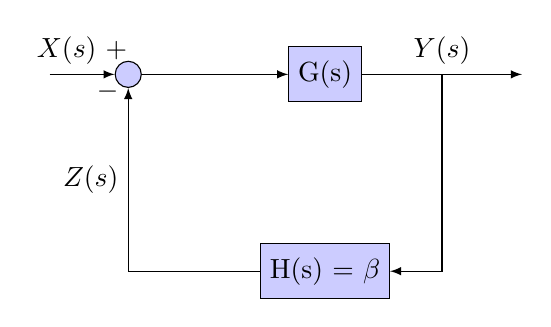
\begin{tikzpicture}[auto, node distance=2.5cm,>=latex]
    % We start by placing the blocks
    \node [input, name=input] {};
    \node [sum, right of=input] (sum) {};
    \node [block, right of=sum] (controller) {G(s)};
    \node [output, right of=controller] (output) {};
    \node [block, below of=controller] (measurements) {H(s) =  $\beta$ };

    \draw [draw,->] (input) -- node {$X(s)\  +$} (sum);
    \draw [->] (sum) -- node {} (controller);
    \draw [->] (controller) -- node [name=y] {$Y(s)$}(output);
    \draw [->] (y) |- (measurements);
    \draw [->] (measurements) -| node[pos=0.99] {$-$} 
        node [near end] {$Z(s)$} (sum);
\end{tikzpicture}
%\end{figure}

